\subsection{DNN Training and Testing}
We train a neural network model across a set of 30 completed runs on 
the track seen in Figure~\ref{fig:track} by a human pilot. Half of 
the runs saw the car driving one way along the track, while the 
remaining half were of the car driving in the opposite direction on 
the track. In total, we collected 2,556 frames for training and 2,609 
frames for validation. In each training step, we use a batch size of 
100 frames which are used to further develop the model. We do this 
across 2,000 training steps. When a model was trained with the 
aformentioned data, the training loss was 0.0188 and the validation 
loss was 0.0132. The change of the loss value over the course of model training can be seen in Figure~\ref{fig:modelloss}.

\begin{figure}[h]
  \centering
  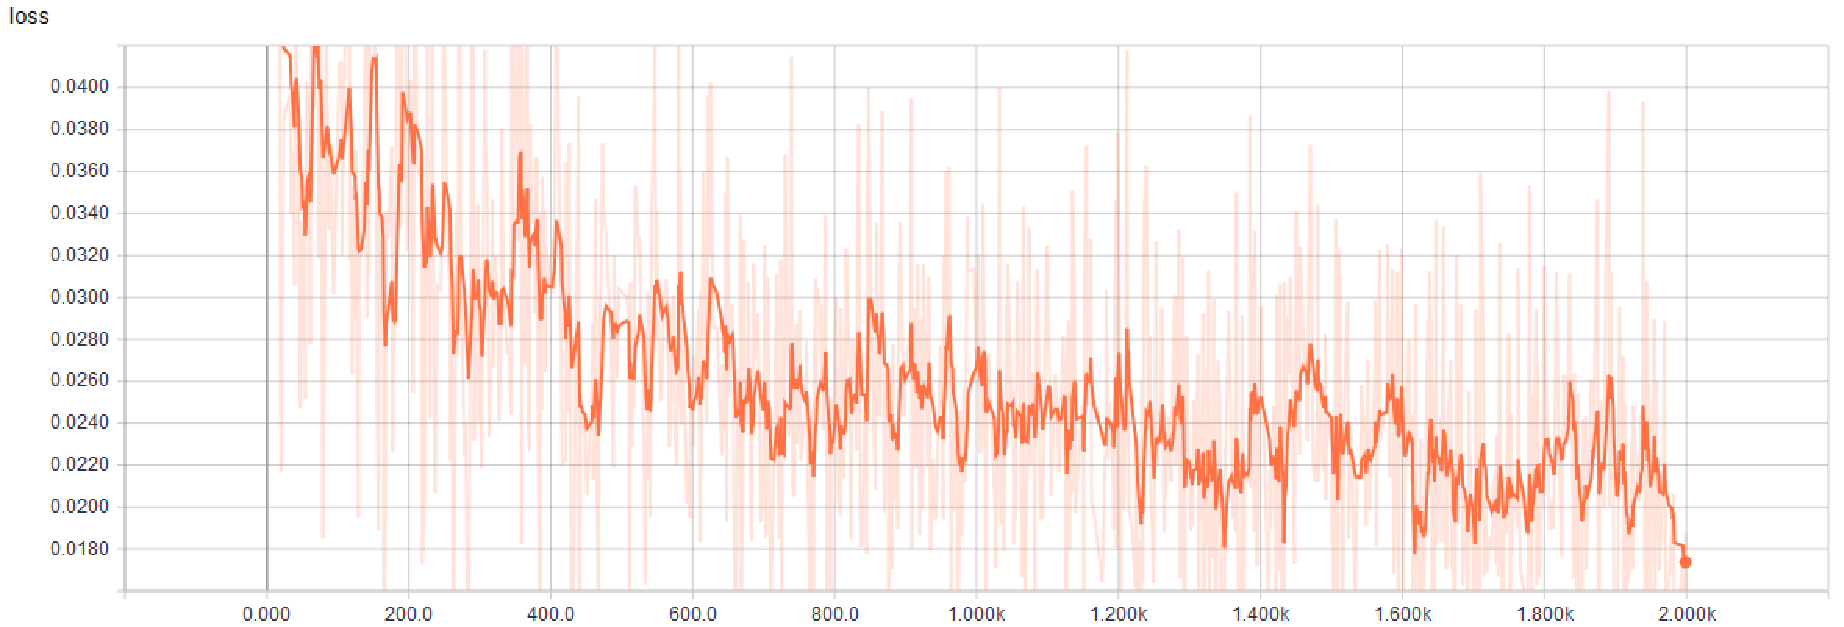
\includegraphics[width=.5\textwidth]{figs/TrainingLoss}
  \caption{Change in loss value throughout training.}
  \label{fig:modelloss}
\end{figure}

We also trained models where center frames (where the car was going 
straight) and curve frames (where the car was turning) were equally 
selected in each batch, and were pleasantly surprised at the change 
in the car's performance. With the second method, the car displayed a 
greater ability to stay in the center of the track (on the white 
tape). This was problematic, however, as the loss values changed with 
the training loss being 0.009 and the validation loss becoming 
0.0869, indicating that overfitting had become a problem. We believe, 
though, that this can be rectified through the collection of 
additional data for training and validation.

\begin{figure}[h]
  \centering
  \includegraphics[width=.55\textwidth]{figs/graph_run=.pdf}
  \caption{ Network visualization. }
  \label{fig:}
\end{figure}
\fixme{Is all of the network graph necessary or only certain parts?}

\subsection{System-level Factors Affecting Real-Time Performance}
In the utilization of the Raspberry Pi 3 in our platform, there are a
few factors that need to be considered and/or enforced in order to
guarantee that the Pi is able to consistently perform at a desired
level. Specifically, these issues all have the potential to negatively
affect the cpu clock speed/frequency, which would result in decreased
performance. While, in the above experiments, the cpu operated at a
preferred clock speed of 1.2 GHz, it is entirely possible for the cpu
to operate at a lower frequency if the following problems are not
taken into account. 

The most notable issue that can affect the cpu clock speed is that of
the power supplied to the Raspberry Pi. In essence, it is necessary
that the Pi be supplied with 2 Amps, as any less could hinder the Pi's
ability to maintain a 1.2 GHz frequency. In experiments conducted with
a power supply that only provided 1 Amp, the Pi was unable to sustain
a 1.2 GHz clock speed and, instead, fluctuated between operating at
600 MHz and 1.2 GHz. As a result, it is necessary, or at least highly
recommended, that the power supply used for the Raspberry Pi 3 be
capable of outputting 2 Amps, otherwise optimal performance isn't
guaranteed.

Another factor that can affect clock speed is that of the
cpu's temperature. Some model operations can be computationally
intensive, thus it is possible for the temperature of the cpu to
become relatively high. This can be especially problematic in
situations where multiple models are running  simultaneously on the
Pi. Consequently, thermal throttling may be used to decrease the clock
speed so that the cpu temperature stays at a safe level. Thus the
Raspberry Pi may not be suited for prolonged use, especially in cases
where the workload is relatively larger, such as running multiple
models. Rather, the Pi seems to be better suited for running in set
periods, after which it is turned  off or made idle so that the cpu is
allowed time to cool down. 

